\documentclass{article}
\usepackage[utf8]{inputenc}

% \usepackage{listings}
\usepackage[utf8]{inputenc}
\usepackage{indentfirst}
\usepackage{graphicx}
\usepackage{hyperref}
\usepackage{caption}
\usepackage{listings}

\usepackage[linesnumbered,lined,commentsnumbered]{algorithm2e}
\usepackage{subcaption}
\usepackage{multirow}
\usepackage{amsmath}
\usepackage{xcolor}
\usepackage{wrapfig}
\usepackage{booktabs,caption,threeparttable}
\usepackage{subcaption}
\usepackage{amsfonts}
\usepackage{amssymb}
\usepackage{array}
\usepackage{xcolor}
\usepackage{wrapfig,lipsum,booktabs}
\usepackage[a4paper, total={6.5in, 8.5in}]{geometry}
\usepackage{setspace}
\usepackage{pdflscape}
\usepackage{tabu}
\usepackage{biblatex} %Imports biblatex package
\linespread{1.25}
\usepackage[breakable, theorems, skins]{tcolorbox}

% \tcbset{enhanced}

\graphicspath{ {./} }

\title{SEL}
\author{Vicol Valeriu}
\date{March 2022}


\begin{document}
% \bibliographystyle{plain}

\DeclareRobustCommand{\mybox}[2][gray!20]{%
\begin{tcolorbox}[   %% Adjust the following parameters at will.
        breakable,
        left=0pt,
        right=0pt,
        top=0pt,
        bottom=0pt,
        colback=#1,
        colframe=#1,
        width=\dimexpr\textwidth\relax, 
        enlarge left by=0mm,
        fontupper=\small, fontlower=\Large,
        boxsep=5pt,
        arc=0pt,outer arc=0pt,
        ]
        #2
\end{tcolorbox}
}


\begin{titlepage}
    \centering
   \sc \LARGE
   \vspace{3cm}
   
\includegraphics[height=4cm,width=4cm]{media/logo.png}\\
   \vspace{1cm}
   Supervised and experiential learning\\ 

   \vfill
   \textbf{Practical Work 1}\\

   \vspace{2cm}
   \Large \vfill
   Valeriu Vicol 
   
   \vfill
 
  Barcelona, \today
\end{titlepage}
\thispagestyle{empty}
\tableofcontents
\vfill
\vspace{.75cm}
\setcounter{page}{1}
\newpage
\section{Introduction}
The purpose of this practical work is to gain practical knowledge  rule induction algorithms, in case of this work is the RISE
algorithm \cite{domingos1996unifying}, which represent a way of unifying the instance-based and rule-based induction
algorithms. Bellow we can find in depth descriptions of how current implementation is structure and why it is done in this way.
\section{Rise classifier}
Main concept of RISE is to create a set of rule from the instance and then try to extend the boundaries/constraints of the rules
in order to increase the precision of rules-set, the process is continuous until the precision is not increasing anymore.

\subsection{Structure}
In Figure \ref{fig:class_structure} we can see the class structure of the classifier, algorithm was implemented mainly 
using object-oriented programming \cite{rentsch1982object} style instead of keeping everything in array and there are few reasons for that. First
reason is that is easier to read for humans which is the most important thing for program, second is that if we would keep everything
in the array it would be hard to maintain the code and to extend it and also with object-oriented programming we can improve the 
performance of the code of the algorithm: 

\begin{itemize}
    \item \path{RiseClassifier}: represents the core class of algorithms which contains the classifier implementation with some 
    data processing functions
    \item \path{RiseUtils}: represents the utils class of algorithms which is computing distance between instance and rules, this logic
    was moved to another class instead of \path{RiseClassifier} as we can experiment with improvements and distances without touching the
    core logic of classifier.
    \item \path{Instance}: represent the instance from the dataset in OOP format
    \item \path{GenericInstanceAttribute}: represent an abstract class which define a property on the instance, we look at this 
    class like an contract definition which will be used across the program.
        \begin{itemize}
        \item \path{NumericalInstanceAttribute}: represent the concrete implementation, with some 
        logic related to numerical attributes of the instance.
        \item \path{CategoricalInstanceAttribute}: represent the concrete implementation, with some 
        logic related to categorical attributes of the instance, which are ordinal encoded beforehand.
        \end{itemize}
    \item \path{InstanceRule}: represent the rule inducted from instance class is similar to \path{Instance}
    except it has more utils method which are computing the distance and extending rule
    \item \path{GenericAttributeRule}: represent abstract class which define a concrete rule for concrete
    attribute
    \begin{itemize}
        \item \path{NumericalInstanceAttribute}: represent the concrete implementation, with some 
        logic related to numerical attributes of the instance.
        \item \path{CategoricalInstanceAttribute}: represent the concrete implementation, with some 
        logic related to categorical attributes of the instance, which are ordinal encoded beforehand.
        \end{itemize}
  \end{itemize}
 There are few more classes which are not included in schema as they are not related to the core algorithm but to 
 data processing.
\begin{figure}[htbp]
    \centering
    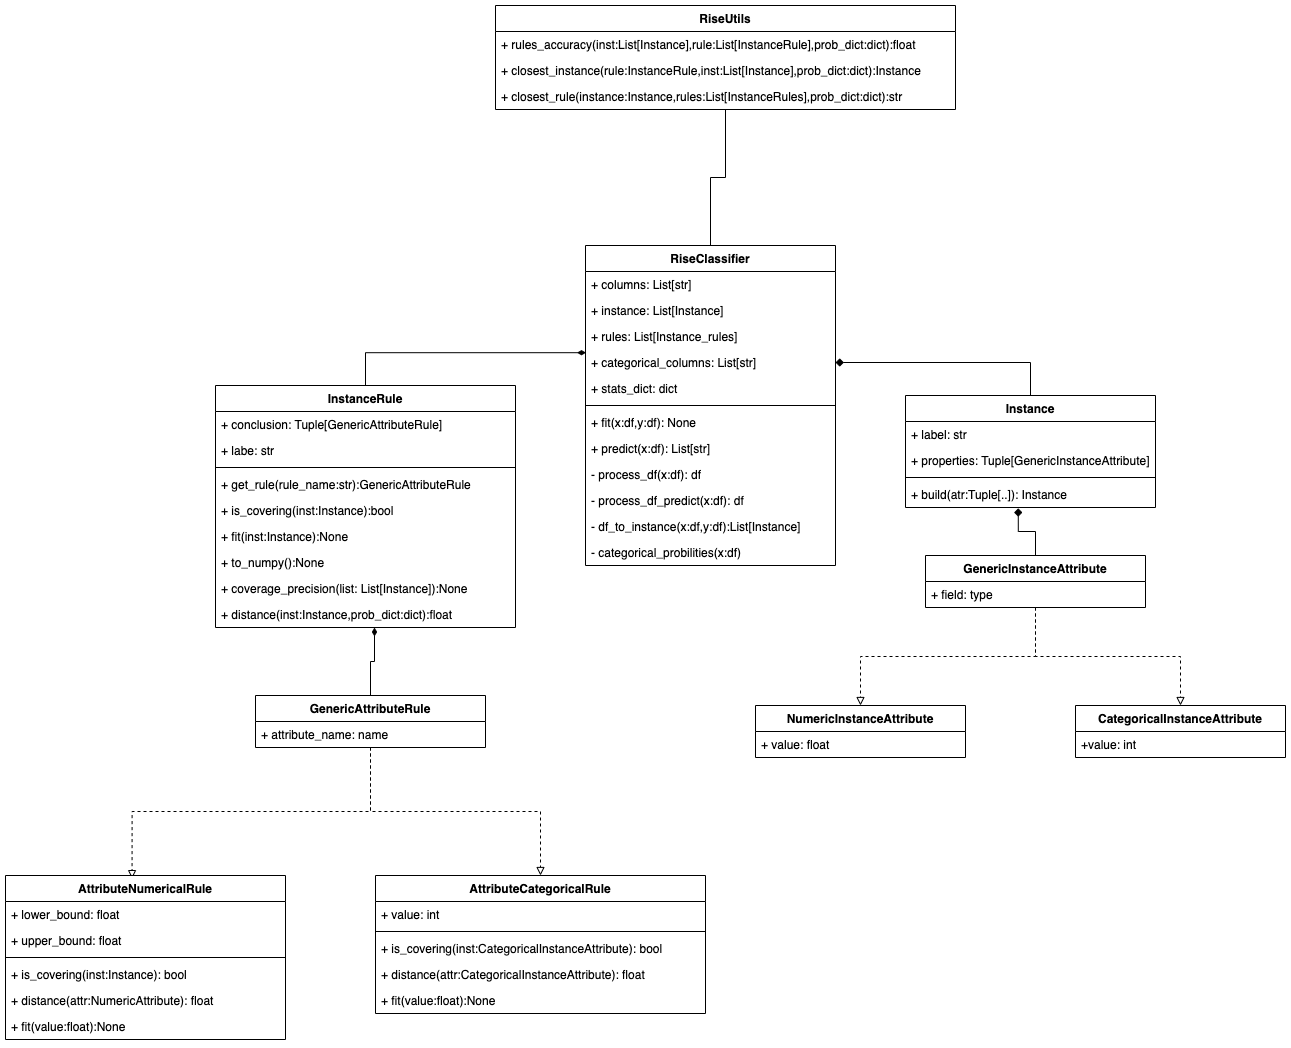
\includegraphics[width=0.9\textwidth]{media/sel.png}
    \caption{Rise classifier class structure}
    \label{fig:class_structure}
\end{figure}








\subsection{Implementation}
In current section we will discuss implementation of the algorithm, in Algorithm \ref{rise_alg} we can see the pseudocode
implementation of the algorithm, there are few minor changes to original implementation, but the idea is similar, in this 
implementation we use more explicit description of the steps. On extra step added is index validation when we remove
the rule from the rule set, as we perform removing of the rule by index we have to take into account this details. Also
were implemented some minor improvements to the original implementation which are discussed in the next section.
Main motivation for changing the algorithm is speed, one of the problems is that we compute many times same distance which
is taking time.

\begin{algorithm}[h!]
    \setlength{\algomargin}{0.5cm}
    \setstretch{1.15}
    \SetKwData{Left}{left}
    \SetKwData{This}{this}\SetKwData{Up}{up}
    \SetKwFunction{Union}{Union}
    \SetKwFunction{FindCompress}{FindCompress}
    \SetKwInOut{Input}{input}
    \SetKwInOut{Output}{output}
    \SetKwFor{While}{while}{:}{end}
    
    \Input{dataframe with the instances and dataframe with the labels}
    \Output{a set of rules inferred from the dataframe}
    \BlankLine
    
    normalization with min-max scaller, and ordinal encoding for categorical values\;
    $instances \gets$ \textbf{df\_to\_instances}$(dataframe,labels)$\;
    $stat\_dict \gets $ \textbf{categorical\_probabilites}$(dataframe,labels)$\;
    $rules \gets set([$InstanceRule$(it) $  for  $  it  $ in $ instances])$ \;
    $rules' \gets rules$\;
    $final\_precision \gets $ \textbf{rules\_precision}($rule,instances,stat\_dict)$\;
    \While{ True }{
        $intial\_precision \gets final\_precision$\;
        \ForEach{$index,rule \in$ \textbf{enum}($rules$)}{
            \If{$len(rules) < index$}{
                $break$ \# because during this loop we update $rules$ by removing some rules we have to add this 
                validation
            }
    
            $closest\_instance \gets$ \textbf{closest\_instance}($rule,instances,stat\_dict$)\;
            $rule ' \gets rule$\;
            $rule ' $.fit($closest\_instance$) \# most specific generalization\;
            $rules'[index] \gets rule'$\;
    
            \If{\textbf{rules\_precision}($instances,rules',..$)$\geq$\textbf{rules\_precision}($instances,rules,..$)}{
                \If{$rule' \in rules$}{
                    $rules' \gets rules' - rule'$\;
                }
                $rule \gets rules'$\;
            }
            \Else{
                $rules'[index] \gets rule$\;
            }
        }
        $final\_preicision \gets$\textbf{rules\_precision}($instances,rules,stats\_dict$)\;
        \If{$intial\_precision \geq final\_precion$}{
            $break$\;
        }
    
    }
    \caption{Rise classifier}
    \label{rise_alg}
\end{algorithm}

\subsection{Improvements}
One major difference between original algorithm and current implementation is caching  the distance between the rule
and the instance, as we perform many times calculations for finding the closest instance to the rule. In current implementation
each rule have a dict with the hash of the instance and distance to it, like this when we have a rule have to calculate the distance
between the instance it tries tot find it in the dict with hashes if is not present there it performs the calculations 
and then save distance and hash of instance in the dict. This small extra step decrease the time of execution significantly.

\newpage
\section{Datasets}
For testing the algorithm were picked 3 different datasets with different size, algorithms have categorical and numerical attributes as for first dataset was picked wine
because it is relatively small, and it has only numerical attributes, similar thing is with second choice as it also mainly contains the numerical attributes and one categorical.
And the third dataset is seismic bumps which contains plenty of numerical attributes and categorical. 

\subsection{Data processing}
As the preprocessing step were used only 2 steps, normalization of numerical attributes using MinMaxScaller and encoding categorical ones using OrdinalEncoder. We 
don't have any missing attributes in datasets, so we don't have to add additional step of filling in missing attributes. Then using StratifiedKFold from sklearn
library dataset was split in 3 folds, so we can train algorithm more than one time on the dataset so see how it is behaves.
\subsection{Wine}
In this section we analyze the results of the algorithm on wine dataset in the Table \ref{table:wine_train} we can see
the results of algorithm on the train set, we can clearly see that algorithm has very good results as all the metrics
are more than 99\%, yes algorithm is overfitting, but we think that is inevitable for all rule induction algorithms to 
overfit the train instances. Next step is to evaluate algorithm on the test set in Table \ref{table:wine_test} we can
observe the results, and again we can clearly say that algorithm has good results, even though in fold 2 and 3, results 
decreased, but all metrics are around 90\% which is a good result.  \\

\begin{table}[h]
    \footnotesize
    \subcaptionbox{fold 1}{
        \begin{tabular}[t]{|p{2.5cm}|c|}
            \hline
            \textbf{metric}& \textbf{value}\\ \hline
            balanced accuracy & 99.29 \% \\ \hline
            accuracy    &   99.15  \% \\ \hline
            f1 score & 99.15 \% \\ \hline   
            precision & 99.17 \% \\  \hline
            recall & 99.15 \% \\ \hline   
       
        \end{tabular}}
        \hfill
        \subcaptionbox{fold 2}{
        \begin{tabular}[t]{|p{2.5cm}|c|}
            \hline
            \textbf{metric}& \textbf{value}\\ \hline
            balanced accuracy & 100\%\\ \hline
            accuracy & 100\% \\ \hline
            f1 score & 100\% \\ \hline
            precision & 100\% \\ \hline   
            recall & 100\% \\ \hline

        

        \end{tabular}}
        \hfill
        \subcaptionbox{fold 3}{
            \begin{tabular}[t]{|p{2.5cm}|c|}
                \hline
                \textbf{metric}& \textbf{value}\\ \hline
                balanced accuracy & 100\%\\ \hline
                accuracy & 100\% \\ \hline
                f1 score & 100\% \\ \hline
                precision & 100\% \\ \hline   
                recall & 100\% \\ \hline
    
            \end{tabular}}
        \caption{Metrics of the rise classifier on the train set}
        \label{table:wine_train}
    \end{table}

    \begin{table}[h]
        \footnotesize
        \subcaptionbox{fold 1}{
            \begin{tabular}[t]{|p{2.5cm}|c|}
                \hline
                \textbf{metric}& \textbf{value}\\ \hline
                balanced accuracy & 94.44 \% \\ \hline
                accuracy    &   93.33  \% \\ \hline
                f1 score & 93.21 \% \\ \hline   
                precision & 94.01 \% \\  \hline
                recall & 93.33 \% \\ \hline   
           
            \end{tabular}}
            \hfill
            \subcaptionbox{fold 2}{
            \begin{tabular}[t]{|p{2.5cm}|c|}
                \hline
                \textbf{metric}& \textbf{value}\\ \hline
                balanced accuracy & 89.8\%\\ \hline
                accuracy & 89.83\% \\ \hline
                f1 score & 89.86\% \\ \hline
                precision & 91.09\% \\ \hline   
                recall & 89.83\% \\ \hline
    
            
    
            \end{tabular}}
            \hfill
            \subcaptionbox{fold 3}{
                \begin{tabular}[t]{|p{2.5cm}|c|}
                    \hline
                    \textbf{metric}& \textbf{value}\\ \hline
                    balanced accuracy & 88.52\%\\ \hline
                    accuracy & 89.83\% \\ \hline
                    f1 score & 89.74\% \\ \hline
                    precision & 91.04\% \\ \hline   
                    recall & 89.83\% \\ \hline
        
                \end{tabular}}
            \caption{Metrics of the rise classifier on the test set}
            \label{table:wine_test}
        \end{table}
\newpage
Bellow are first 2 and last 2 rules inducted by the rise classifier from the dataset. As we can see each rule is 
covering small amount of instances around 1.6\% which is 2-3 instance which, but the precision of are 100\% this results
can be interpreted as each rule knows, few instances and is able to classify them. We can observe this in inferred boundaries
of the rule bellow. One more thing is to mention here the last rules are covering only one instance as we can
see this rule didn't even extend the attributes, the reason why this happens is topic of investigation. \\

\mybox{
    \begin{itemize}
        \item  class[3]  - coverage[1.681\%] -  precision[100.0\%] --  ['(Alcohol in [0.404,0.602])', '(Malic.acid in [0.504,0.549])', '(Ash in [0.32,0.392])', '(Acl in [0.48,0.48])', '(Mg in [0.196,0.196])', '(Phenols in [0.172,0.221])', '(Flavanoids in [0.03,0.068])', '(Nonflavanoid.phenols in [0.5,0.846])', '(Proanth in [0.148,0.177])', '(Color.int in [0.422,0.858])', '(Hue in [0.247,0.34])', '(OD in [0.17,0.196])', '(Proline in [0.215,0.29])']
        \item  class[2]  - coverage[1.681\%] -  precision[100.0\%] -- ['(Alcohol in [0.16,0.16])', '(Malic.acid in [0.004,0.516])', '(Ash in [0.196,0.196])', '(Acl in [0.451,0.451])', '(Mg in [0.174,0.185])', '(Phenols in [0.352,0.497])', '(Flavanoids in [0.274,0.405])', '(Nonflavanoid.phenols in [0.308,0.442])', '(Proanth in [0.322,0.461])', '(Color.int in [0.0,0.117])', '(Hue in [0.464,0.928])', '(OD in [0.649,0.675])', '(Proline in [0.0,0.204])']
        \item  ... ...
        \item class[3]  - coverage[0.847\%] -  precision[100.0\%] -- ['(Alcohol in [0.923,0.923])', '(Malic.acid in [0.755,0.755])', '(Ash in [0.885,0.885])', '(Acl in [0.716,0.716])', '(Mg in [0.321,0.321])', '(Phenols in [0.33,0.33])', '(Flavanoids in [0.088,0.088])', '(Nonflavanoid.phenols in [0.811,0.811])', '(Proanth in [0.369,0.369])', '(Color.int in [0.663,0.663])', '(Hue in [0.106,0.106])', '(OD in [0.125,0.125])', '(Proline in [0.215,0.215])']
		\item  class[1]  - coverage[0.847\%] -  precision[100.0\%] -- ['(Alcohol in [0.902,0.902])', '(Malic.acid in [0.2,0.2])', '(Ash in [0.59,0.59])', '(Acl in [0.278,0.278])', '(Mg in [0.691,0.691])', '(Phenols in [0.678,0.678])', '(Flavanoids in [0.823,0.823])', '(Nonflavanoid.phenols in [0.208,0.208])', '(Proanth in [0.663,0.663])', '(Color.int in [0.347,0.347])', '(Hue in [0.496,0.496])', '(OD in [0.921,0.921])', '(Proline in [0.39,0.39])']

    \end{itemize}
}


\subsection{Breast cancer}
For the breast cancer dataset we can see similar picture as we had in for the wine dataset, but however in the
case of breast cancer algorithm is able to generalize better as we can see in Table \ref{table:cancer_train} and in 
Table \ref{table:cancer_test}. Even though the metrics for train are not 100\% as in wine dataset for the train
but in the test we can clearly see the difference for fold 2 \& 3 we can higher results comparing to the
wine dataset. In file \path{/out/cancer.txt} we have classification report we can see that we  have recall for class Malignant around 96\%, 
which is a good result, but there is space for improvement.

\begin{table}[h]
    \footnotesize
    \subcaptionbox{fold 1}{
        \begin{tabular}[t]{|p{2.5cm}|c|}
            \hline
            \textbf{metric}& \textbf{value}\\ \hline
            balanced accuracy & 99.51 \% \\ \hline
            accuracy    &   99.36  \% \\ \hline
            f1 score & 99.36 \% \\ \hline   
            precision & 99.37 \% \\  \hline
            recall & 99.36 \% \\ \hline   
       
        \end{tabular}}
        \hfill
        \subcaptionbox{fold 2}{
        \begin{tabular}[t]{|p{2.5cm}|c|}
            \hline
            \textbf{metric}& \textbf{value}\\ \hline
            balanced accuracy & 99.53\%\\ \hline
            accuracy & 99.57\% \\ \hline
            f1 score & 99.57\% \\ \hline
            precision & 99.57\% \\ \hline   
            recall & 99.57\% \\ \hline
    

        \end{tabular}}
        \hfill
        \subcaptionbox{fold 3}{
            \begin{tabular}[t]{|p{2.5cm}|c|}
                \hline
                \textbf{metric}& \textbf{value}\\ \hline
                balanced accuracy & 99.67\%\\ \hline
                accuracy & 99.57\% \\ \hline
                f1 score & 99.57\% \\ \hline
                precision & 99.58\% \\ \hline   
                recall & 99.57\% \\ \hline
    
            \end{tabular}}
        \caption{Metrics of the rise classifier on the train set}
        \label{table:cancer_train}
    \end{table}

    \begin{table}[h]
        \footnotesize
        \subcaptionbox{fold 1}{
            \begin{tabular}[t]{|p{2.5cm}|c|}
                \hline
                \textbf{metric}& \textbf{value}\\ \hline
                balanced accuracy & 94.29\%\\ \hline
                accuracy & 94.85\% \\ \hline
                f1 score & 94.85\% \\ \hline
                precision & 94.85\% \\ \hline   
                recall & 94.85 \% \\ \hline
            \end{tabular}}
            \hfill
            \subcaptionbox{fold 2}{
            \begin{tabular}[t]{|p{2.5cm}|c|}
                \hline
                \textbf{metric}& \textbf{value}\\ \hline
                balanced accuracy & 96.46\%\\ \hline
                accuracy & 96.14\% \\ \hline
                f1 score & 96.16\% \\ \hline
                precision & 96.29\% \\ \hline   
                recall & 96.14 \% \\ \hline
            \end{tabular}}
            \hfill
            \subcaptionbox{fold 3}{
                \begin{tabular}[t]{|p{2.5cm}|c|}
                    \hline
                    \textbf{metric}& \textbf{value}\\ \hline
                    balanced accuracy & 95.64\%\\ \hline
                    accuracy & 96.57\% \\ \hline
                    f1 score & 96.55\% \\ \hline
                    precision & 96.59\% \\ \hline
                    ine   
                    recall & 96.57\% \\ \hline
        
                \end{tabular}
            }
            \caption{Metrics of the rise classifier on the test set}
            \label{table:cancer_test}
        \end{table}
Bellow we can see the inferred rule from the dataset one major difference is coverage comparing to wine dataset, but this difference is more related to size of the dataset. 
Also, we can see that second rule coverage is 6.87\% and has 100\% which is impressive if we compare with the last rules which 
have about 0.2\% coverage.  \\
\mybox{
    \begin{itemize}
    \item  class[Malignant]  - coverage[0.429\%] -  precision[100.0\%] -- ['(Clump Thickness in [1.0,1.0])', '(Uniformity of Cell Size in [0.444,0.778])', '(Uniformity of Cell Shape in [0.667,0.778])', '(Marginal Adhesion in [0.333,0.333])', '(Single Epithelial Cell Size in [0.333,1.0])', '(Bare Nuclei == 1.0)', '(Bland Chromatin in [0.778,0.778])', '(Normal Nucleoli in [0.0,0.889])', '(Mitoses in [0.0,0.0])']
    \item class[Benign]  - coverage[6.867\%] -  precision[100.0\%] -- ['(Clump Thickness in [0.111,0.444])', '(Uniformity of Cell Size in [0.0,0.0])', '(Uniformity of Cell Shape in [0.0,0.0])', '(Marginal Adhesion in [0.0,0.0])', '(Single Epithelial Cell Size in [0.111,0.111])', '(Bare Nuclei == 0.0)', '(Bland Chromatin in [0.111,0.111])', '(Normal Nucleoli in [0.0,0.0])', '(Mitoses in [0.0,0.0])']
    \item ... ... 
    \item class[Malignant]  - coverage[0.215\%] -  precision[100.0\%] -- ['(Clump Thickness in [1.0,1.0])', '(Uniformity of Cell Size in [0.222,0.222])', '(Uniformity of Cell Shape in [0.556,0.556])', '(Marginal Adhesion in [0.111,0.111])', '(Single Epithelial Cell Size in [0.222,0.222])', '(Bare Nuclei == 5.0)', '(Bland Chromatin in [0.333,0.333])', '(Normal Nucleoli in [1.0,1.0])', '(Mitoses in [0.111,0.111])']
    \item class[Malignant]  - coverage[0.215\%] -  precision[100.0\%] -- ['(Clump Thickness in [0.778,0.778])', '(Uniformity of Cell Size in [1.0,1.0])', '(Uniformity of Cell Shape in [1.0,1.0])', '(Marginal Adhesion in [1.0,1.0])', '(Single Epithelial Cell Size in [0.444,0.444])', '(Bare Nuclei == 1.0)', '(Bland Chromatin in [0.778,0.778])', '(Normal Nucleoli in [1.0,1.0])', '(Mitoses in [0.556,0.556])']
    \end{itemize}
}

\subsection{Obesity}

\section{Conclusion}
As part of this practical work we implemented the rise classification algorithm which represent a way of unifying the 
instance-based learning and rule induction algorithms. As we saw in previous sections we can achieve great results
with rise, but major problem in my opinion is the speed of algorithm because the training time is taking great amount of time
for big datasets. For further work should be investigated any ways of improving the speed of the algorithm like
avoid computing more than one time distance between rule and instance, this is the main pain point in main opinion, because
this is done when we want to extend a rule or get the precision of rule-set which is costly. Work around with hashing
values of instance decreased the execution for wine set from 400 seconds to 12 seconds, but however the amount of time for
big datasets is high. For more in-depth investigation of the results we can check the output files in the \path{output} directory
where can see complete image of output of the algorithm. 

% \addbibresource{refs.bib}



\end{document}